\subsubsection{Equipment}
\begin{itemize}
    \item Hot plate 
    \item Plastic cup  
    \item Digital thermocouple 
    \item Magnetic stirrer  
    \item Cotton wool 
    \item Aluminium foil 
    \item Scissors 
    \item Tape 
\end{itemize}
\subsubsection{Method} \label{sec:Heating-method}
To find out which insulator is better out of aluminium foil and cotton, an experiment was conducted as follow: 
\begin{enumerate}
    \item Wrapped the cup with cotton jacket. Set the hot plate at 100\si{\celsius} with \SI{300}{\cubic\centi\meter} of water in the cup and measure the time taken for it to reach \SI{33}{\celsius}.
    \item Repeat step one with aluminium wrapped around the cup. 
    To find out the effect of heat conduction, experiments were conducted as follow: 
    \item Mark dots at regular intervals using ruler along the bottom and side of the cup.  
    \item The plastic cup was then placed on the hot plate, which is set at 35\si{\celsius} and the temperature was measured and recorded at different positions using dots marked. No insulation and mixing method were used. Horizontal measurements taken at 0 cm, 1.5 cm and 3 cm from the side of the cup towards the centre. Vertical measurements taken at 1.5 cm, 4.5 cm and 7.5 cm from bottom to the top of the cup. All horizontal measurements were taken at a vertical distance of 7.5 cm as the impeller system was in the cup therefore could not be taken at the bottom of the cup. 
    \item Repeat step 4 under mixing condition using a magnetic stirrer. 
    \item Repeat step 5 with insulation layer around the cup using 1cm thick cotton.  
    \item Repeat step 5 with insulation layer around the cup using 2cm thick cotton.   
    \item Repeat step 7 with an aluminium foil layer on top of the cup. 
    \item Results of the temperature at each point were recorded on tables in section 4. 
\end{enumerate}
 

\begin{figure}[h]
    \centering
    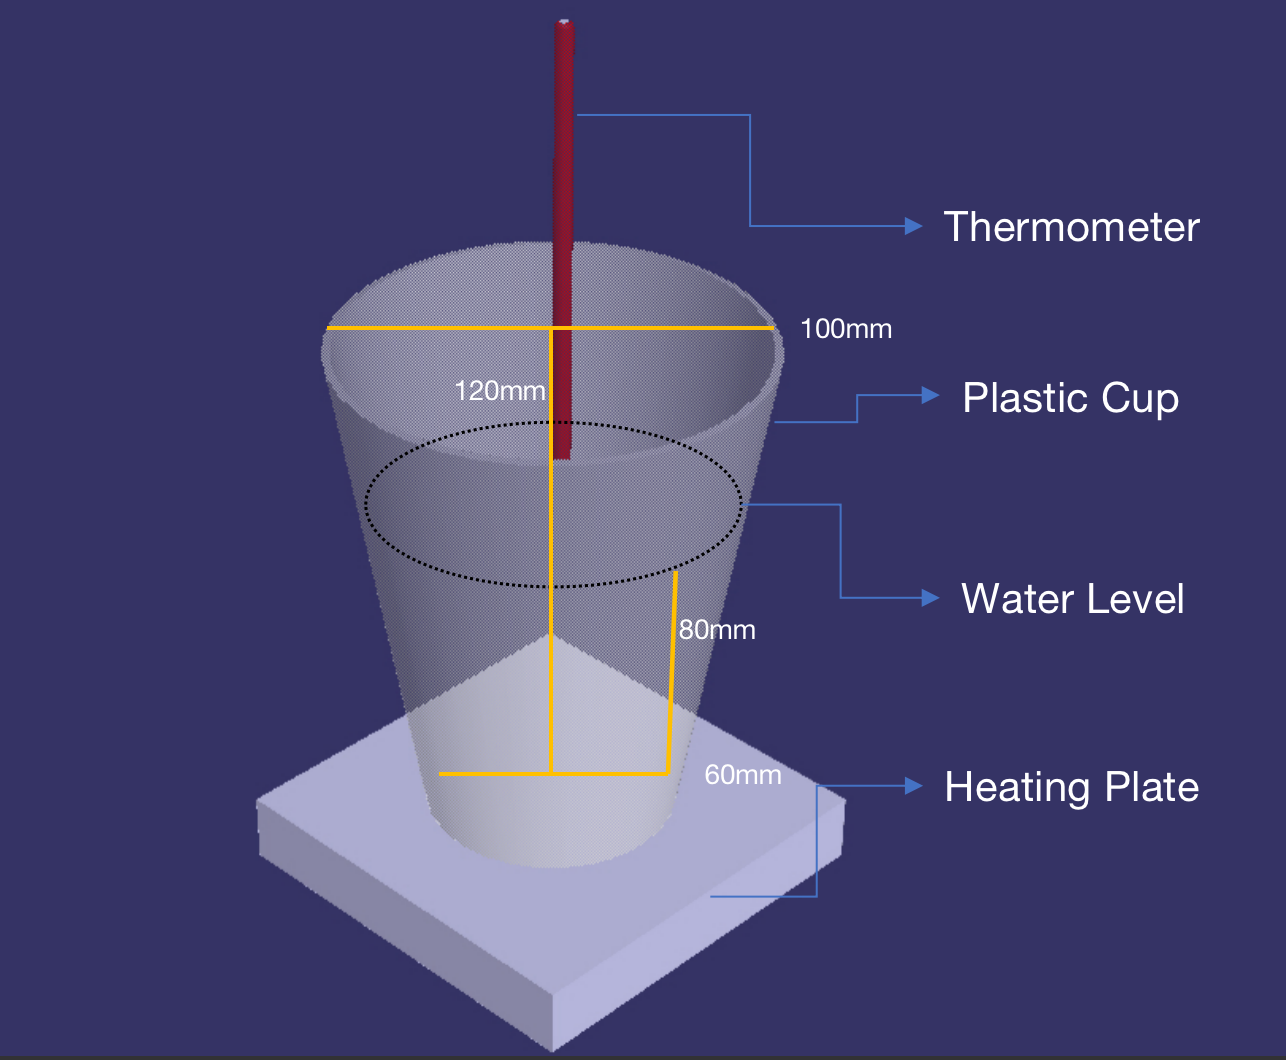
\includegraphics[width=0.40\textwidth]{Heating-cup.png}
    \caption{Apparatus setup}
    \label{}
\end{figure}